\documentclass[landscape,a0paper,fontscale=0.3]{baposter}

\usepackage{times}
\usepackage{calc}
\usepackage{url}
\usepackage{graphicx}
\usepackage{amsthm}
\usepackage{amsmath}
\usepackage{amssymb}
\usepackage{relsize}
\usepackage{multirow}
\usepackage{multicol}
\usepackage{booktabs}
\usepackage{microtype}
\usepackage{graphicx}

\usepackage[T1]{fontenc}
\usepackage{ae}
\usepackage{enumitem}
\usepackage{colortbl}
\usepackage{xcolor}
\usepackage{tcolorbox}
\usepackage[vlined]{algorithm2e}
\usepackage{minted}

\setlength{\algomargin}{0pt}

\setlist[itemize]{leftmargin=*,nosep}
\setlength{\columnsep}{0.7em}
\setlength{\columnseprule}{0mm}

\setlist[enumerate]{leftmargin=2.3em,nosep}
\setlength{\columnsep}{0.5em}
\setlength{\columnseprule}{0mm}

% \renewcommand{\rmdefault}{ptm} % Arial
% \renewcommand{\sfdefault}{ptm} % Arial
\renewcommand{\familydefault}{\sfdefault}

\begin{document}

\begin{poster}{
 % Show grid to help with alignment
 grid=false,
 columns=4,
 % Column spacing
 colspacing=0.7em,
 % Color style
 headerColorOne=cyan!20!white!90!black,
 borderColor=cyan!30!white!90!black,
 % Format of textbox
 textborder=faded,
 % Format of text header
 headerborder=open,
 headershape=roundedright,
 headershade=plain,
 background=none,
 bgColorOne=cyan!10!white,
 headerheight=0.15\textheight}
 % Eye Catcher
 {
    \makebox[0.01\textwidth]{}
    
\includegraphics[width=0.07\linewidth]{figs/buaa.png}
    
\includegraphics[width=0.12\linewidth]{figs/uottawa.png}
 }
 % Title
 {\sc\huge\bf Regularizing Neural Networks via Adversarial Model Perturbation}
 % Authors
 {\vspace{0.5em} Yaowei Zheng,\textsuperscript{1} Richong Zhang,\textsuperscript{1} Yongyi Mao\textsuperscript{2} \\[0.5em]
 {\textsuperscript{1}BDBC and SKLSDE, Beihang University, Beijing, China\\[0.2em]
  \textsuperscript{2}School of EECS, University of Ottawa, Ottawa, Canada}}
 % University logo
 {
  \begin{tabular}{r}
    \makebox[0.02\textwidth]{}
    
\includegraphics[width=0.15\linewidth]{figs/cvprlogo.png}
    \makebox[0.01\textwidth]{}
  \end{tabular}
 }


\headerbox{\bf\color{blue}Summary}{name=summary,column=0,row=0,span=1}{
\textbf{\color{blue}Background:} Effective regularization schemes are highly desired in deep learning for alleviating overfitting and improving generalization.\\
\textbf{\color{blue}Motivation:} Previous work suggested that flat minima can improve generalization both in theoretical and empirical perspectives [1-4]. \\
\textbf{\color{blue}Contribution:} We propose Adversarial Model Perturbation (AMP) as a powerful regularization scheme principled by the objective of finding flat minima, which achieves better classification performance and calibration results.\\
\begin{minipage}{0.99\linewidth}
\centering
\begin{minipage}{0.4\linewidth}
\centering
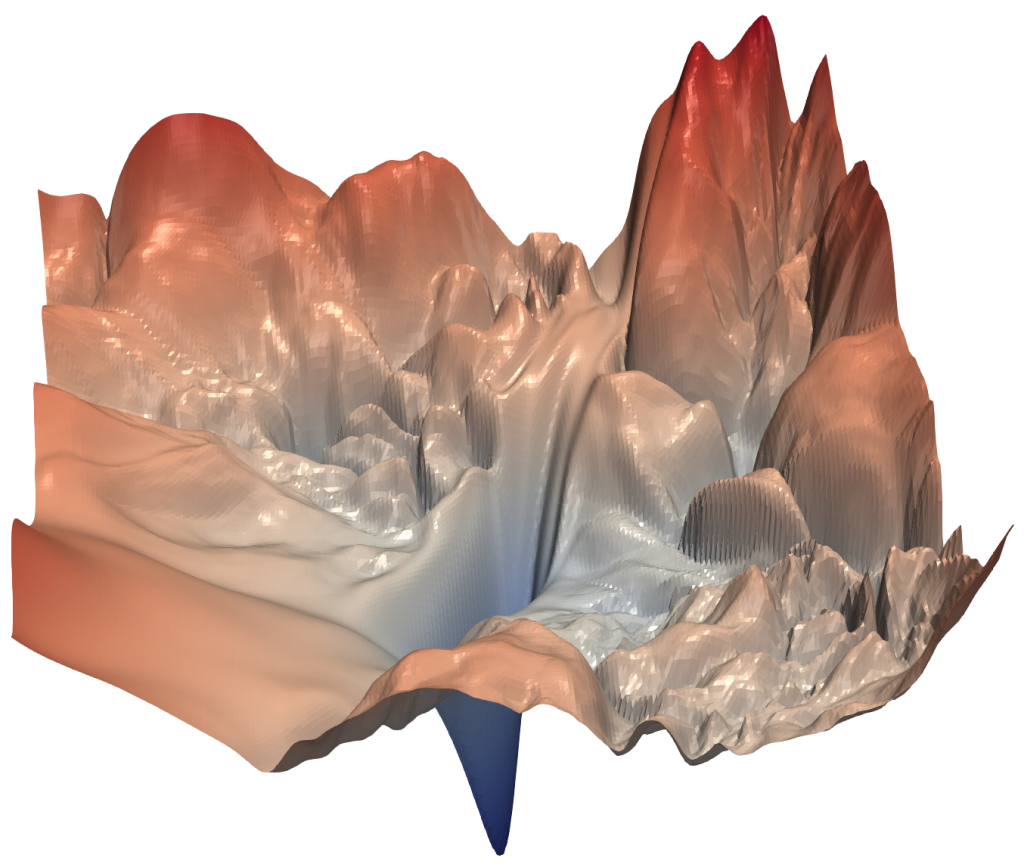
\includegraphics[width=.65\linewidth]{figs/flatness_a.png}
\end{minipage}
\begin{minipage}{0.4\linewidth}
\centering
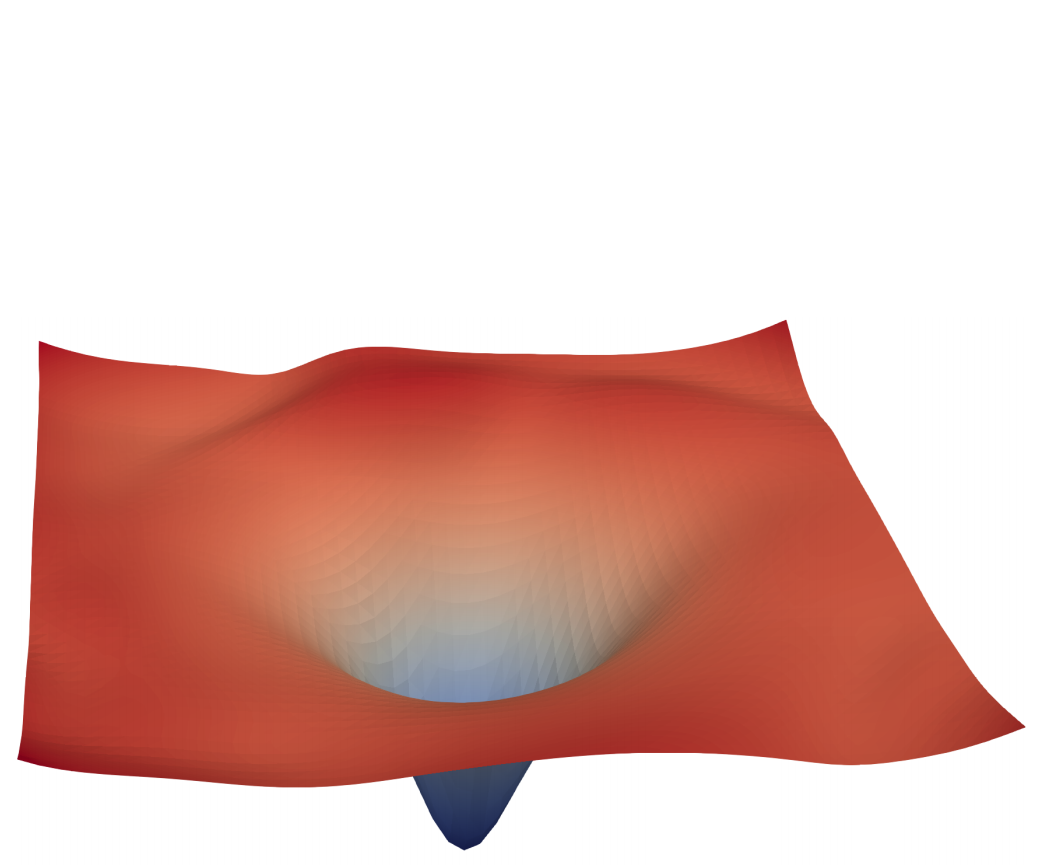
\includegraphics[width=.65\linewidth]{figs/flatness_b.png}
\end{minipage}

\vspace{0.5em}
(Better minima are flatter, visualized by Li \textit{et al}., 2018.)\\
\end{minipage}
}

%%%%%%%%%%%%%%%%%%%%%%%%%%%%%%%%%%%%%%%%%%%%%%%%%%%%%%%%%%%%%%%%%%%%%%%%%%%%%
\headerbox{\bf\color{blue}Method}{name=method,column=1,row=0,span=1}{
\textbf{\color{blue}AMP: Adversarial Model Perturbation}\\
We derive an AMP loss from the empirical risk (ERM loss) by applying the ``worst'' perturbation on the model parameters to penalize the sharp minima.\\
\vspace{-0.5em}
\begin{equation*}
\mathcal{L}_\mathrm{ERM}(\boldsymbol{\theta}):=\frac{1}{|D|}\sum_{(\boldsymbol{x},\boldsymbol{y})\in\mathcal{D}}\ell(\boldsymbol{x},\boldsymbol{y};\boldsymbol{\theta})
\end{equation*}
\begin{equation*}
\mathcal{L}_\mathrm{AMP}(\boldsymbol{\theta}):=\max_{\Delta:\Vert\Delta\Vert\le\epsilon}\mathcal{L}_\mathrm{ERM}(\boldsymbol{\theta}+\Delta)
\end{equation*}
It can be seen as an analogue of a ``max-pooling'' operation on the empirical risk on each point in the parameter space.\\
\begin{minipage}{0.99\linewidth}
\centering
\begin{minipage}{0.4\linewidth}
\centering
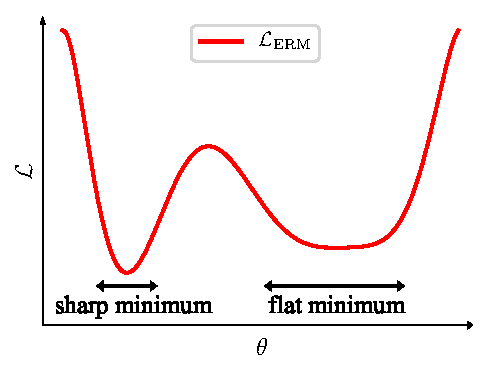
\includegraphics[width=.9\linewidth]{figs/loss_example_a.pdf}
\end{minipage}
\begin{minipage}{0.4\linewidth}
\centering
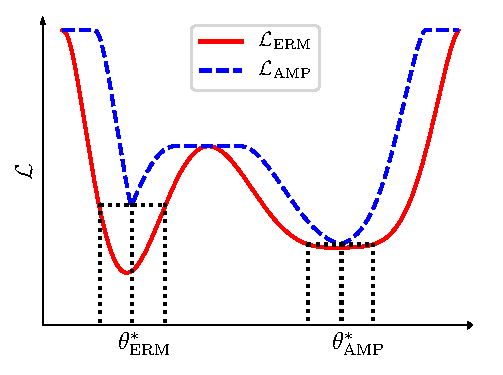
\includegraphics[width=.9\linewidth]{figs/loss_example_b.pdf}
\end{minipage}
\end{minipage}
}

%%%%%%%%%%%%%%%%%%%%%%%%%%%%%%%%%%%%%%%%%%%%%%%%%%%%%%%%%%%%%%%%%%%%%%%%%%%%%
\headerbox{\bf\color{blue}Experiments}{name=results,column=2,row=0,span=2}{
\begin{minipage}{0.9\linewidth}
\textbf{\color{blue}Results on Image Classification Benchmarks:}
\vspace{0.5em}
\end{minipage}

\begin{minipage}{0.33\linewidth}
\centering
\resizebox{.95\linewidth}{!}{%
\begin{tabular}{lcc}
\toprule
PreActResNet18 & Test Error (\%) & Test NLL \\
\midrule
ERM & 2.95$\pm$0.063 & 0.166$\pm$0.004 \\
Dropout & 2.80$\pm$0.065 & 0.156$\pm$0.012 \\
Label Smoothing & 2.78$\pm$0.087 & 0.998$\pm$0.002 \\
Flooding & 2.84$\pm$0.047 & \underline{0.130$\pm$0.003} \\
MixUp & \underline{2.74$\pm$0.044} & 0.146$\pm$0.004 \\
Adv. Training & 2.77$\pm$0.080 & 0.151$\pm$0.018 \\
RMP & 2.93$\pm$0.066 & 0.161$\pm$0.010 \\
AMP & \textbf{2.30$\pm$0.025} & \textbf{0.096$\pm$0.002} \\
\midrule
VGG16 & Test Error (\%) & Test NLL \\
\midrule
ERM & 3.14$\pm$0.060 & 0.140$\pm$0.027 \\
Dropout & 2.96$\pm$0.049 & 0.134$\pm$0.027 \\
Label Smoothing & 3.07$\pm$0.070 & 1.004$\pm$0.002 \\
Flooding & 3.15$\pm$0.085 & 0.128$\pm$0.003 \\
MixUp & 3.09$\pm$0.057 & 0.160$\pm$0.003 \\
Adv. Training & \underline{2.94$\pm$0.091} & \underline{0.122$\pm$0.003} \\
RMP & 3.19$\pm$0.052 & 0.134$\pm$0.004 \\
AMP & \textbf{2.73$\pm$0.015} & \textbf{0.116$\pm$0.006} \\
\bottomrule
\end{tabular}
}

\vspace{0.5em}
(a) SVHN
\vspace{0.5em}
\end{minipage}
\begin{minipage}{0.33\linewidth}
\centering
\resizebox{.95\linewidth}{!}{%
\begin{tabular}{lcc}
\toprule
PreActResNet18 & Test Error (\%) & Test NLL \\
\midrule
ERM & 5.02$\pm$0.212 & 0.239$\pm$0.009 \\
Dropout & 4.86$\pm$0.148 & 0.223$\pm$0.009 \\
Label Smoothing & 4.85$\pm$0.115 & 1.038$\pm$0.003 \\
Flooding & 4.97$\pm$0.082 & \underline{0.166$\pm$0.003} \\
MixUp & \underline{4.09$\pm$0.117} & 0.198$\pm$0.004 \\
Adv. Training & 4.99$\pm$0.085 & 0.247$\pm$0.006 \\
RMP & 4.97$\pm$0.167 & 0.239$\pm$0.008 \\
AMP & \textbf{3.97$\pm$0.091} & \textbf{0.129$\pm$0.003} \\
\midrule
VGG16 & Test Error (\%) & Test NLL \\
\midrule
ERM & 6.32$\pm$0.193 & 0.361$\pm$0.012 \\
Dropout & 6.22$\pm$0.147 & 0.314$\pm$0.009 \\
Label Smoothing & 6.29$\pm$0.158 & 1.076$\pm$0.003 \\
Flooding & 6.26$\pm$0.145 & \underline{0.234$\pm$0.005} \\
MixUp & \textbf{5.48$\pm$0.112} & 0.251$\pm$0.003 \\
Adv. Training & 6.49$\pm$0.130 & 0.380$\pm$0.010 \\
RMP & 6.30$\pm$0.109 & 0.363$\pm$0.010 \\
AMP & \underline{5.65$\pm$0.147} & \textbf{0.207$\pm$0.005} \\
\bottomrule
\end{tabular}
}

\vspace{0.5em}
(b) CIFAR-10
\vspace{0.5em}
\end{minipage}
\begin{minipage}{0.33\linewidth}
\centering
\resizebox{.95\linewidth}{!}{%
\begin{tabular}{lcc}
\toprule
PreActResNet18 & Test Error (\%) & Test NLL \\
\midrule
ERM & 24.31$\pm$0.303 & 1.056$\pm$0.013 \\
Dropout & 24.48$\pm$0.351 & 1.110$\pm$0.021 \\
Label Smoothing & 22.07$\pm$0.256 & 2.099$\pm$0.005 \\
Flooding & 24.50$\pm$0.234 & 0.950$\pm$0.011 \\
MixUp & \underline{21.78$\pm$0.210} & \underline{0.910$\pm$0.007} \\
Adv. Training & 25.23$\pm$0.229 & 1.110$\pm$0.012 \\
RMP & 24.28$\pm$0.138 & 1.059$\pm$0.011 \\
AMP & \textbf{21.51$\pm$0.308} & \textbf{0.774$\pm$0.016} \\
\midrule
VGG16 & Test Error (\%) & Test NLL \\
\midrule
ERM & 27.84$\pm$0.297 & 1.827$\pm$0.209 \\
Dropout & 27.72$\pm$0.337 & 1.605$\pm$0.062 \\
Label Smoothing & 27.49$\pm$0.179 & 2.310$\pm$0.005 \\
Flooding & 27.93$\pm$0.271 & 1.221$\pm$0.037 \\
MixUp & \underline{26.81$\pm$0.254} & \underline{1.136$\pm$0.013} \\
Adv. Training & 29.12$\pm$0.145 & 1.535$\pm$0.389 \\
RMP & 27.81$\pm$0.327 & 1.873$\pm$0.035 \\
AMP & \textbf{25.60$\pm$0.168} & \textbf{1.049$\pm$0.049} \\
\bottomrule
\end{tabular}
}

\vspace{0.5em}
(c) CIFAR-100
\vspace{0.5em}
\end{minipage}

\begin{minipage}{0.6\linewidth}
\textbf{\color{blue}Improvement over Various Data Augmentation Techniques:}
\vspace{0.5em}
\end{minipage}
\begin{minipage}{0.39\linewidth}
\textbf{{\color{blue}Calibration Results:} (lower is better)}
\vspace{0.5em}
\end{minipage}

\begin{minipage}{0.6\linewidth}
\centering
\resizebox{.9\linewidth}{!}{%
\begin{tabular}{llcccc}
\toprule
Test Error (\%) & Augment & \multicolumn{2}{c}{WideResNet-28-10} & \multicolumn{2}{c}{PyramidNet-164-270}\\
Dataset & Technique & ERM & AMP & ERM & AMP \\
\midrule
 & Vanilla & 2.57$\pm$0.067 & \textbf{2.19$\pm$0.036} & 2.47$\pm$0.034 & \textbf{2.11$\pm$0.041} \\
SVHN & Cutout & 2.27$\pm$0.085 & \textbf{1.83$\pm$0.018} & 2.19$\pm$0.021 & \textbf{1.82$\pm$0.023} \\
 & AutoAug & 1.91$\pm$0.059 & \textbf{1.61$\pm$0.024} & 1.80$\pm$0.044 & \textbf{1.35$\pm$0.056} \\
\midrule
 & Vanilla & 3.87$\pm$0.167 & \textbf{3.00$\pm$0.059} & 3.60$\pm$0.197 & \textbf{2.75$\pm$0.040} \\
CIFAR-10 & Cutout & 3.38$\pm$0.081 & \textbf{2.67$\pm$0.043} & 2.83$\pm$0.102 & \textbf{2.27$\pm$0.034} \\
 & AutoAug & 2.78$\pm$0.134 & \textbf{2.32$\pm$0.097} & 2.49$\pm$0.128 & \textbf{1.98$\pm$0.062} \\
\midrule
 & Vanilla & 19.17$\pm$0.270 & \textbf{17.33$\pm$0.110} & 17.13$\pm$0.210 & \textbf{15.09$\pm$0.092} \\
CIFAR-100 & Cutout & 18.12$\pm$0.114 & \textbf{16.04$\pm$0.071} & 16.45$\pm$0.136 & \textbf{14.34$\pm$0.153} \\
 & AutoAug & 17.79$\pm$0.185 & \textbf{14.95$\pm$0.088} & 15.43$\pm$0.269 & \textbf{13.36$\pm$0.245} \\
\bottomrule
\end{tabular}
}
\end{minipage}
\begin{minipage}{0.39\linewidth}
\centering
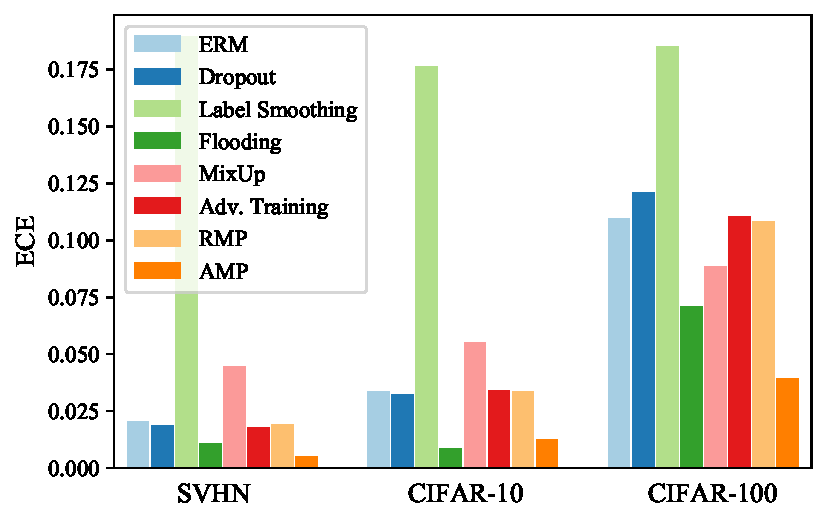
\includegraphics[width=.95\linewidth]{figs/ece.pdf}
\end{minipage}

\begin{minipage}{0.49\linewidth}
\vspace{0.5em}
\textbf{\color{blue}Flatness of the Selected Minima:}
\vspace{0.5em}
\end{minipage}
\begin{minipage}{0.5\linewidth}
\vspace{0.5em}
\textbf{\color{blue}Loss Values with Varying Perturbation Size:}
\vspace{0.5em}
\end{minipage}

\begin{minipage}{0.49\linewidth}
\begin{minipage}{0.5\linewidth}
\centering
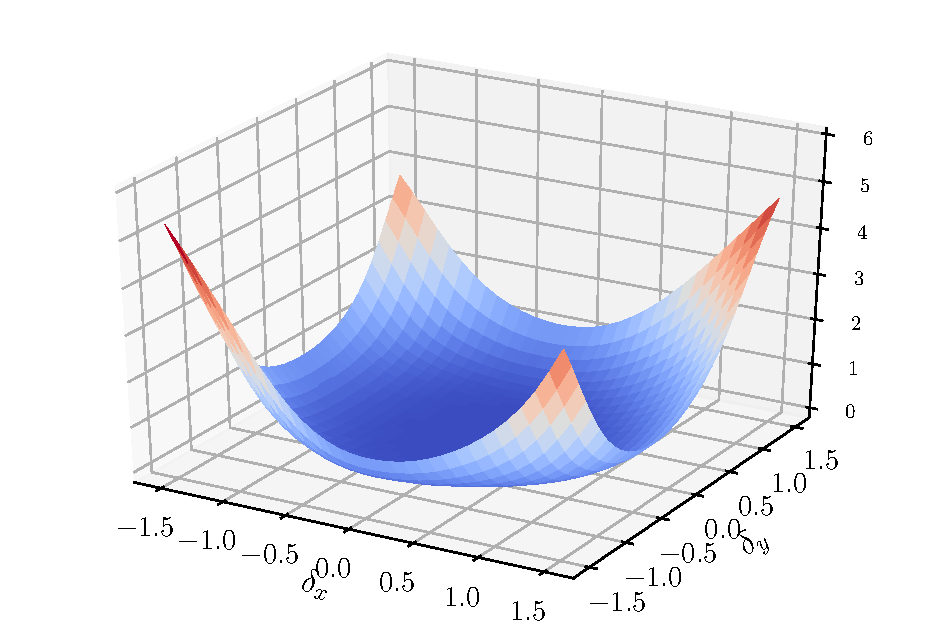
\includegraphics[width=.99\linewidth]{figs/svhn_erm_train_loss_landscape3D.pdf}
\vspace{0.5em}
ERM Training Loss
\vspace{1em}
\end{minipage}
\begin{minipage}{0.49\linewidth}
\centering
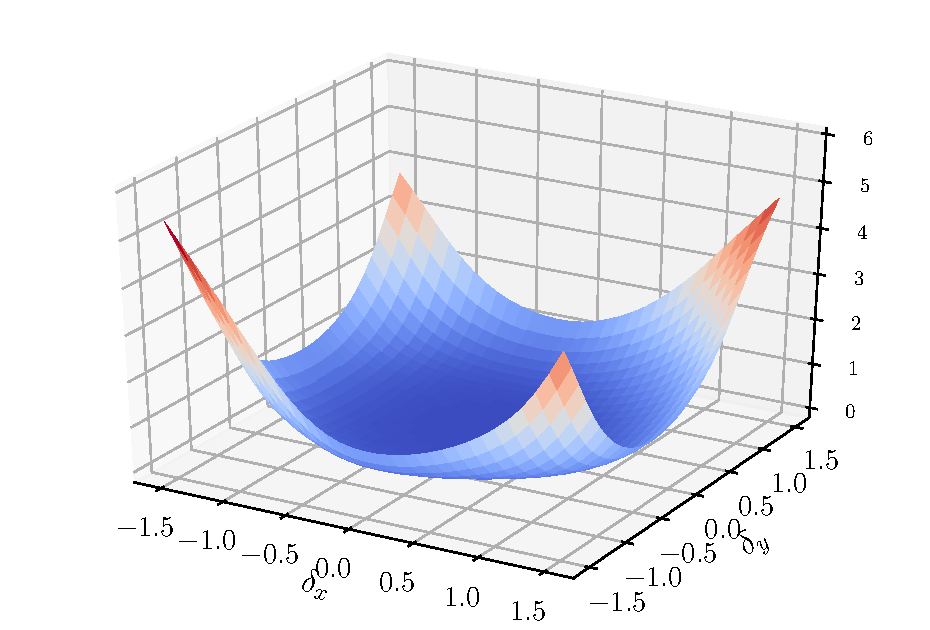
\includegraphics[width=.99\linewidth]{figs/svhn_erm_test_loss_landscape3D.pdf}
\vspace{0.5em}
ERM Test Loss
\vspace{1em}
\end{minipage}

\begin{minipage}{0.5\linewidth}
\centering
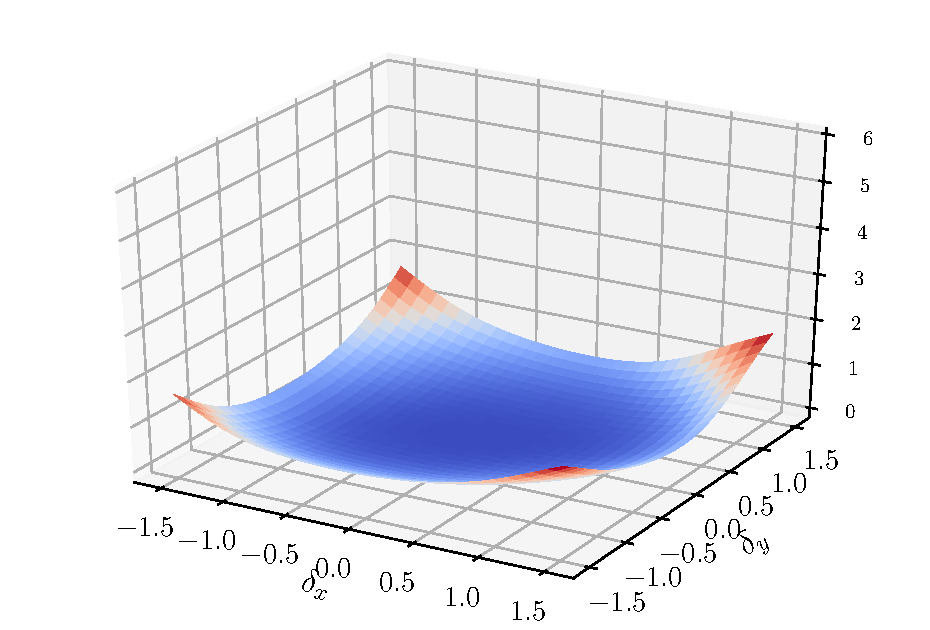
\includegraphics[width=.99\linewidth]{figs/svhn_amp_train_loss_landscape3D.pdf}
\vspace{0.5em}
AMP Training Loss
\vspace{1em}
\end{minipage}
\begin{minipage}{0.49\linewidth}
\centering
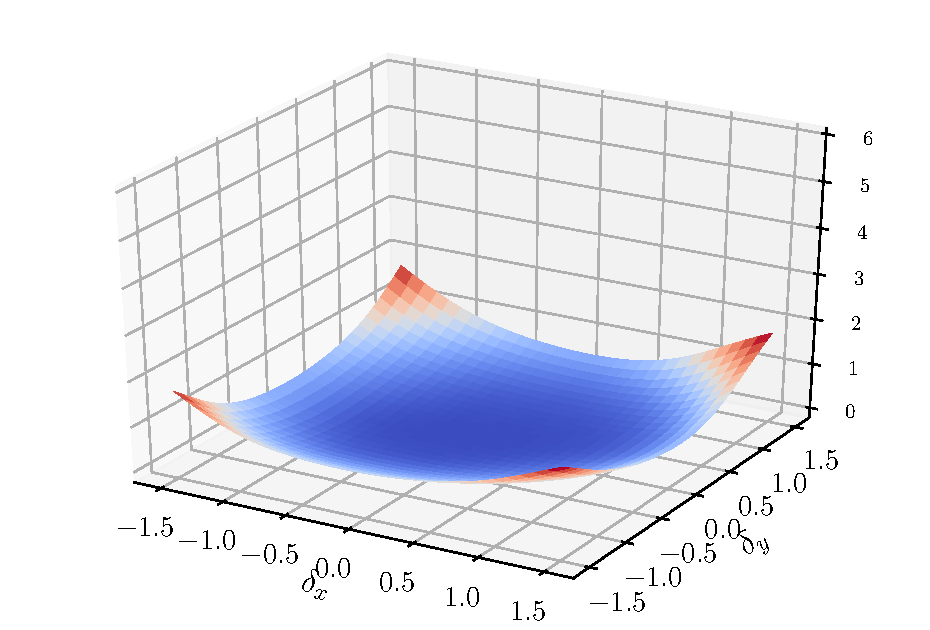
\includegraphics[width=.99\linewidth]{figs/svhn_amp_test_loss_landscape3D.pdf}
\vspace{0.5em}
AMP Test Loss
\vspace{1em}
\end{minipage}
\end{minipage}
\begin{minipage}{0.5\linewidth}
\begin{minipage}{0.5\linewidth}
\centering
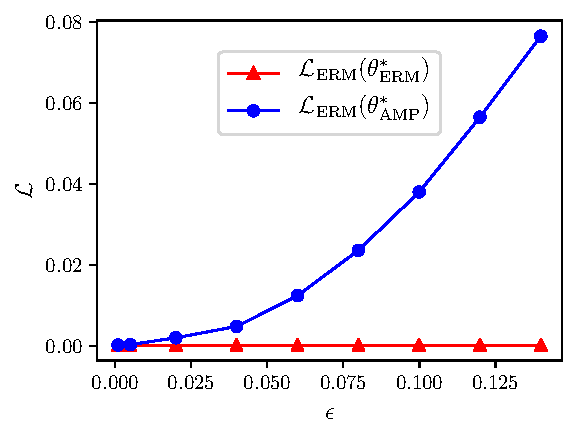
\includegraphics[width=.95\linewidth]{figs/tune_a.pdf}
(a) CIFAR-10 Training Set
\vspace{1em}
\end{minipage}
\begin{minipage}{0.49\linewidth}
\centering
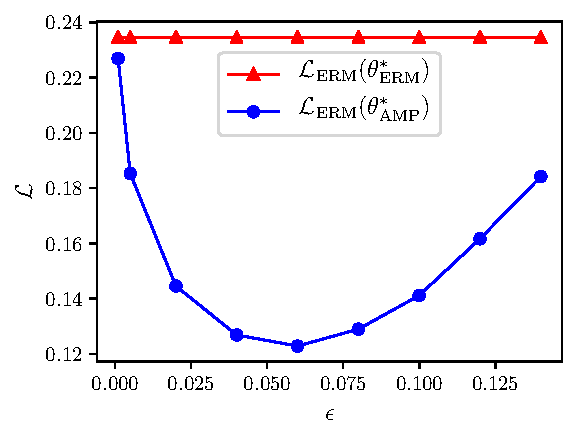
\includegraphics[width=.95\linewidth]{figs/tune_b.pdf}
(b) CIFAR-10 Test Set
\vspace{1em}
\end{minipage}
\textbf{\color{blue}References:}\\
\vspace{-1em}
\begin{enumerate}[label={[\arabic*]}]
    \item Hochreiter \textit{et al}. Flat minima. Neural Computation, 9(1):1-42, 1997.
    \item Keskar \textit{et al}. On large-batch training for deep learning: Generalization gap and sharp minima. In ICLR, 2017.
    \item Li \textit{et al}. Visualizing the loss landscape of neural nets. In NeurIPS, 2018.
    \item Foret \textit{et al}. Sharpness-aware minimization for efficiently improving generalization. In ICLR, 2021.
\end{enumerate}
\end{minipage}
}


%%%%%%%%%%%%%%%%%%%%%%%%%%%%%%%%%%%%%%%%%%%%%%%%%%%%%%%%%%%%%%%%%%%%%%%%%%%%%
\headerbox{\bf\color{blue}Training~Algorithm}{name=algorithm,column=0,below=summary,span=1}{
\textbf{\color{blue}Optimization Objective:}
\vspace{-0.5em}
\begin{equation*}
\min_{\boldsymbol{\theta}}\max_{\Delta:\Vert\Delta\Vert\le\epsilon}\mathcal{L}_\mathrm{ERM}(\boldsymbol{\theta}+\Delta)
\end{equation*}
\vspace{-1.5em}

\textbf{\color{blue}Pseudo-code:}
\begin{tcolorbox}[colframe=blue,colback=white,boxrule=0.5pt,arc=4pt,left=6pt,right=0pt,top=2pt,bottom=2pt,boxsep=0pt]
{\small
\begin{algorithm}[H]
\While{$\boldsymbol{\theta}$ not converged}{
Initialize perturbation $\Delta$ with $\boldsymbol{0}$\;
\For{$n\gets1\text{ to }N$}{
Update $\Delta$ to maximize $\mathcal{L}_\mathrm{ERM}(\boldsymbol{\theta}+\Delta)$ via gradient ascent with learning rate $\zeta$\;
\If{$\Vert\Delta\Vert_2>\epsilon$}{
Normalize $\Delta$ to restrict its norm $\Vert\Delta\Vert_2$ to $\epsilon$;
}
}
Update $\boldsymbol{\theta}$ to minimize $\mathcal{L}_\mathrm{ERM}(\boldsymbol{\theta}+\Delta)$ via gradient descent with learning rate $\eta$\;
}
\end{algorithm}
}
\end{tcolorbox}
\textbf{\color{blue}PyTorch Implementation:}
\begin{tcolorbox}[colframe=blue,colback=white,boxrule=0.5pt,arc=4pt,left=6pt,right=6pt,top=6pt,bottom=6pt,boxsep=0pt]
{\small
\mintinline{python}{from amp import AMP}\\
\mintinline{python}{opt = AMP(params, lr=0.1, epsilon=0.5)}\\
\mintinline{python}{for inputs, targets in dataset:}\\
\makebox[0.05\textwidth]{}\mintinline{python}{def closure():}\\
\makebox[0.10\textwidth]{}\mintinline{python}{opt.zero_grad()}\\
\makebox[0.10\textwidth]{}\mintinline{python}{outputs = model(inputs)}\\
\makebox[0.10\textwidth]{}\mintinline{python}{loss = loss_fn(outputs, targets)}\\
\makebox[0.10\textwidth]{}\mintinline{python}{loss.backward()}\\
\makebox[0.10\textwidth]{}\mintinline{python}{return outputs, loss}\\
\makebox[0.05\textwidth]{}\mintinline{python}{outputs, loss = opt.step(closure)}
}
\end{tcolorbox}
\textbf{\color{blue}Official Code:}\\
\url{https://github.com/hiyouga/AMP-Regularizer}
}


%%%%%%%%%%%%%%%%%%%%%%%%%%%%%%%%%%%%%%%%%%%%%%%%%%%%%%%%%%%%%%%%%%%%%%%%%%%%%
\headerbox{\bf\color{blue}Theoretical~Justification}{name=method,column=1,below=summary,span=1,boxpadding=0.45em}{
\textbf{\color{blue}AMP Finds Flatter Minima:}\\
Assuming that the loss surface of each local minimum in $\!\mathcal{L}_\mathrm{ERM}\!$ can be {\em locally} approximated as an inverted Gaussian surface $\!\gamma\!$ with a mean vector $\!\boldsymbol{\mu}\!$ and a covariance matrix $\!\boldsymbol{\kappa}$.\\
Under the locally Gaussian assumption, the empirical risk $\gamma(\boldsymbol{\theta};\boldsymbol{\mu},\boldsymbol{\kappa},A,C)$ is minimized when $\boldsymbol{\theta}=\boldsymbol{\mu}$ and the minimum value is $\gamma^\ast(\boldsymbol{\mu},\boldsymbol{\kappa},A,C)=C-A$. The minimum value of the AMP loss is the empirical risk at the location in the narrowest principal direction of the cross-section of the loss surface:
\vspace{-1.2em}
\begin{equation*}
\gamma_\mathrm{AMP}^\ast(\boldsymbol{\mu},\boldsymbol{\kappa},A,C)=C-A\exp\left(-\frac{\epsilon^2}{2\sigma^2}\right)
\end{equation*}
\vspace{-1.7em}

\noindent where $\sigma^2$ is the smallest eigenvalue of $\boldsymbol{\kappa}$.\\
It is clear that $\gamma^\ast_\mathrm{AMP}$ although related to the minimum value of empirical risk $\gamma^\ast$, it also takes into account the curvature of the surface around the local minimum.\\
\begin{minipage}{0.99\linewidth}
\centering
\begin{minipage}{0.4\linewidth}
\centering
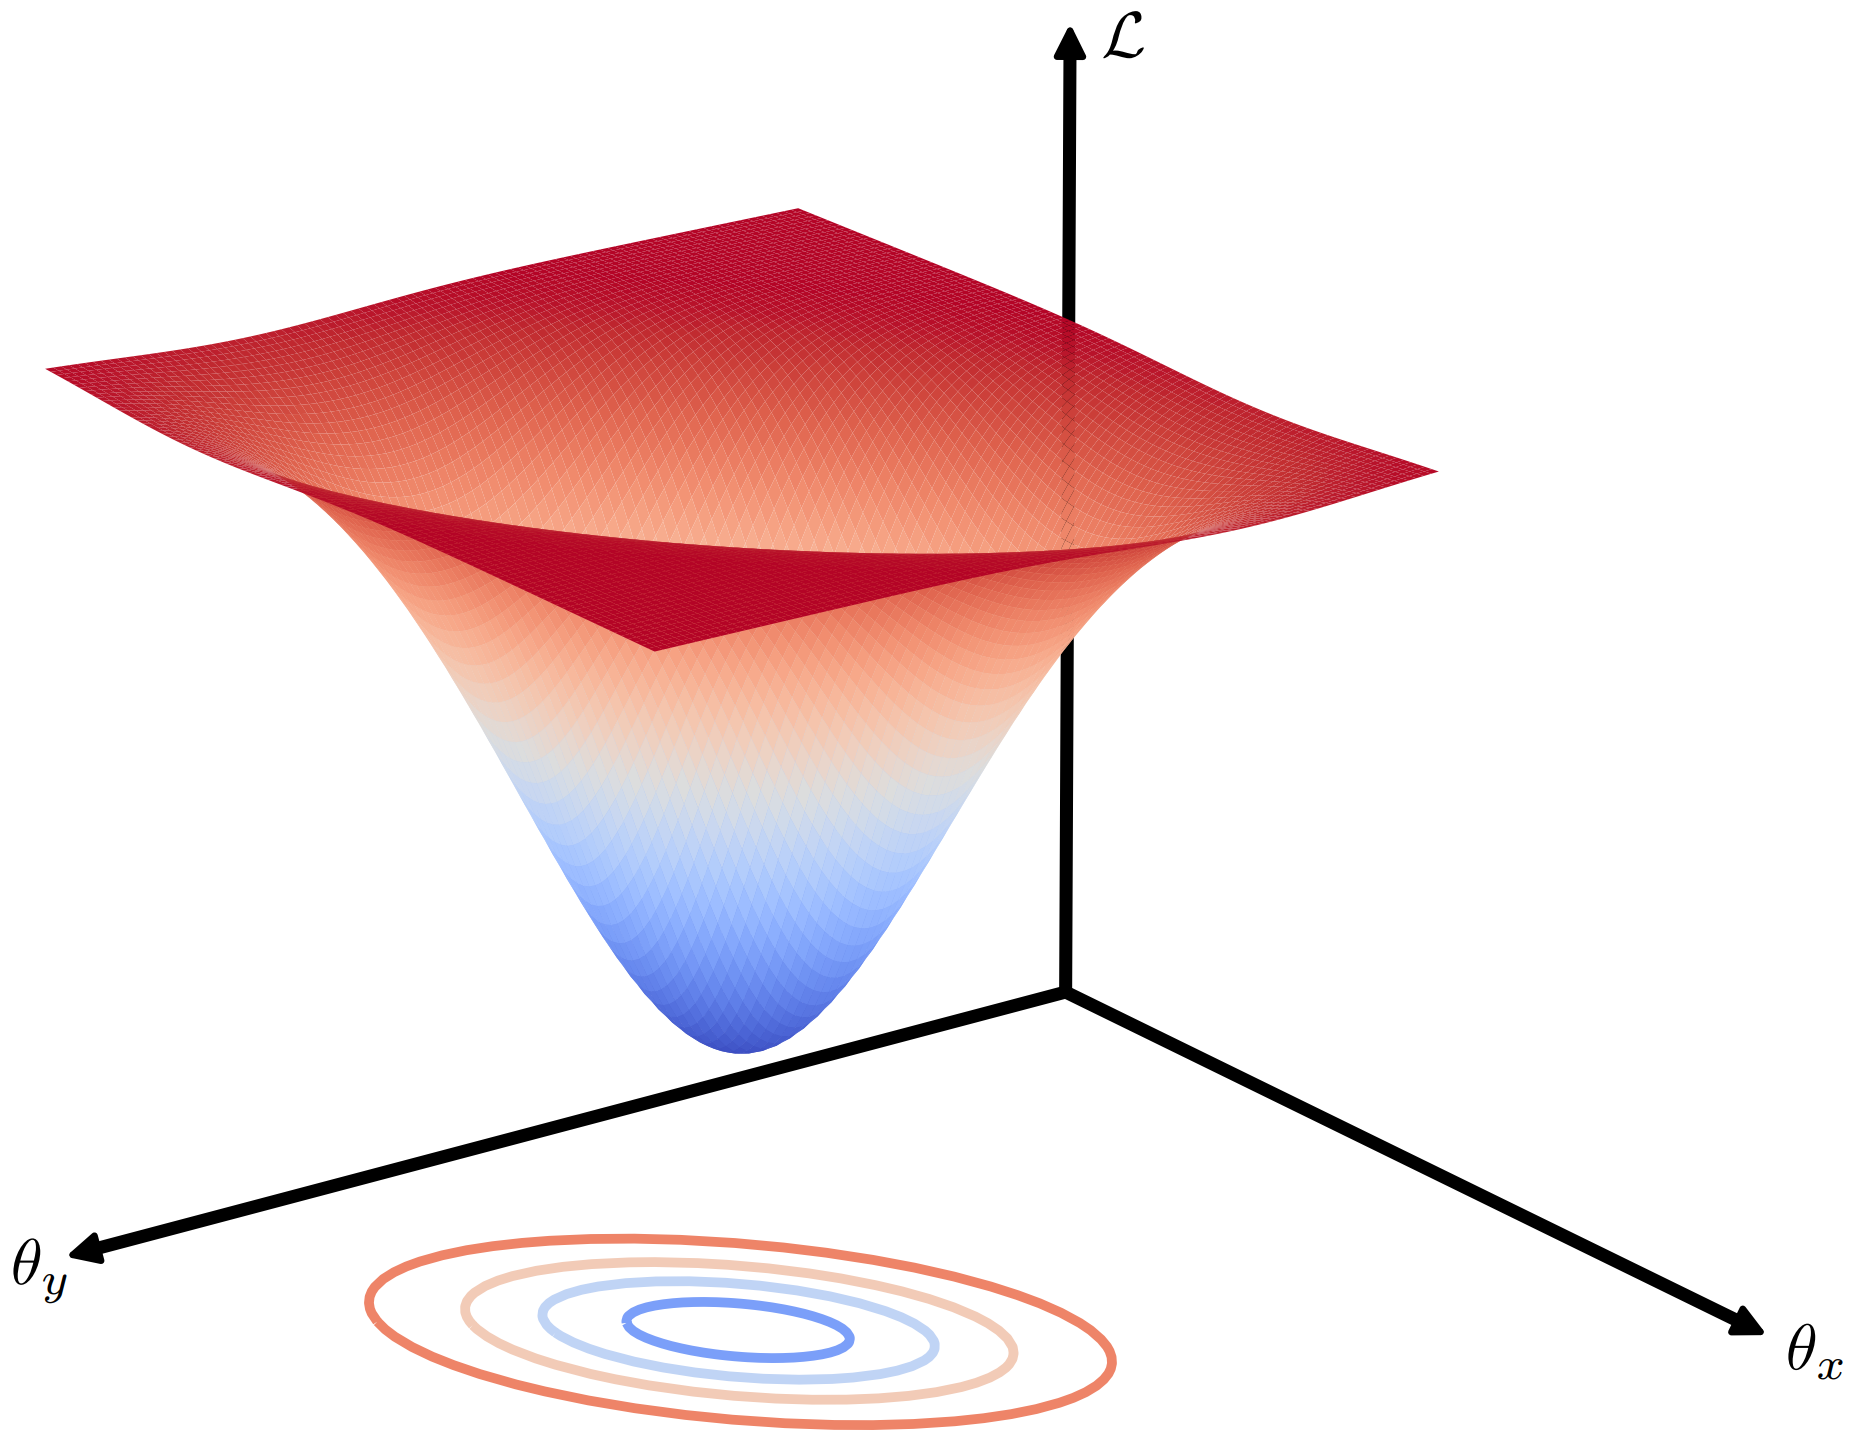
\includegraphics[width=.8\linewidth]{figs/surface.png}
\end{minipage}
\begin{minipage}{0.4\linewidth}
\centering
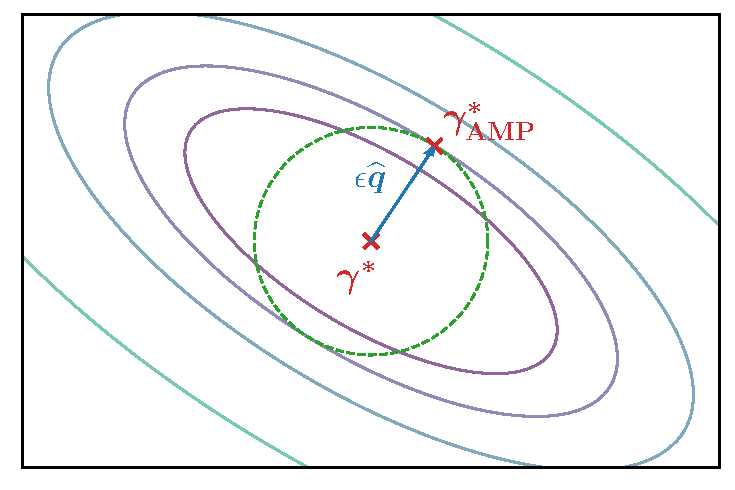
\includegraphics[width=.8\linewidth]{figs/gaussian.pdf}
\end{minipage}
\end{minipage}

\textbf{\color{blue}AMP Regularizes Gradient Norm:}\\
Consider that $N\!=\!1$ (in fact used). The AMP training is equivalent to ERM training with an additional term:
\vspace{-0.8em}
\begin{equation*}
\widetilde{\mathcal{J}}_\mathrm{ERM}(\boldsymbol{\theta}):=\mathcal{J}_\mathrm{ERM}(\boldsymbol{\theta})+\Omega(\boldsymbol{\theta})
\end{equation*}
\vspace{-2.3em}

where
\vspace{-1.1em}
\begin{equation*}
\Omega(\boldsymbol{\theta}):=\begin{cases}
\zeta\Vert\nabla_{\boldsymbol{\theta}}\mathcal{J}_\mathrm{ERM}(\boldsymbol{\theta})\Vert_2^2,&\!\!\!\!\Vert\zeta\nabla_{\boldsymbol{\theta}}\mathcal{J}_\mathrm{ERM}(\boldsymbol{\theta})\Vert_2\le\epsilon\\
\epsilon\Vert\nabla_{\boldsymbol{\theta}}\mathcal{J}_\mathrm{ERM}(\boldsymbol{\theta})\Vert_2,&\!\!\!\!\Vert\zeta\nabla_{\boldsymbol{\theta}}\mathcal{J}_\mathrm{ERM}(\boldsymbol{\theta})\Vert_2>\epsilon
\end{cases}
\end{equation*}
\vspace{-1.5em}

Note that a minimum with smaller gradient norms around it is a flatter minimum.
}

\end{poster}
\end{document}
